\documentclass{article}\usepackage[]{graphicx}\usepackage[]{color}
%% maxwidth is the original width if it is less than linewidth
%% otherwise use linewidth (to make sure the graphics do not exceed the margin)
\makeatletter
\def\maxwidth{ %
  \ifdim\Gin@nat@width>\linewidth
    \linewidth
  \else
    \Gin@nat@width
  \fi
}
\makeatother

\definecolor{fgcolor}{rgb}{0.345, 0.345, 0.345}
\newcommand{\hlnum}[1]{\textcolor[rgb]{0.686,0.059,0.569}{#1}}%
\newcommand{\hlstr}[1]{\textcolor[rgb]{0.192,0.494,0.8}{#1}}%
\newcommand{\hlcom}[1]{\textcolor[rgb]{0.678,0.584,0.686}{\textit{#1}}}%
\newcommand{\hlopt}[1]{\textcolor[rgb]{0,0,0}{#1}}%
\newcommand{\hlstd}[1]{\textcolor[rgb]{0.345,0.345,0.345}{#1}}%
\newcommand{\hlkwa}[1]{\textcolor[rgb]{0.161,0.373,0.58}{\textbf{#1}}}%
\newcommand{\hlkwb}[1]{\textcolor[rgb]{0.69,0.353,0.396}{#1}}%
\newcommand{\hlkwc}[1]{\textcolor[rgb]{0.333,0.667,0.333}{#1}}%
\newcommand{\hlkwd}[1]{\textcolor[rgb]{0.737,0.353,0.396}{\textbf{#1}}}%

\usepackage{framed}
\makeatletter
\newenvironment{kframe}{%
 \def\at@end@of@kframe{}%
 \ifinner\ifhmode%
  \def\at@end@of@kframe{\end{minipage}}%
  \begin{minipage}{\columnwidth}%
 \fi\fi%
 \def\FrameCommand##1{\hskip\@totalleftmargin \hskip-\fboxsep
 \colorbox{shadecolor}{##1}\hskip-\fboxsep
     % There is no \\@totalrightmargin, so:
     \hskip-\linewidth \hskip-\@totalleftmargin \hskip\columnwidth}%
 \MakeFramed {\advance\hsize-\width
   \@totalleftmargin\z@ \linewidth\hsize
   \@setminipage}}%
 {\par\unskip\endMakeFramed%
 \at@end@of@kframe}
\makeatother

\definecolor{shadecolor}{rgb}{.97, .97, .97}
\definecolor{messagecolor}{rgb}{0, 0, 0}
\definecolor{warningcolor}{rgb}{1, 0, 1}
\definecolor{errorcolor}{rgb}{1, 0, 0}
\newenvironment{knitrout}{}{} % an empty environment to be redefined in TeX

\usepackage{alltt}
\usepackage{Sweave}
\usepackage{graphicx}
\usepackage{tabularx}
\usepackage[small]{caption}
\usepackage{gensymb}
\usepackage{float}
\usepackage{subfig}
\usepackage{url}
\setkeys{Gin}{width=0.8\textwidth}
\setlength{\captionmargin}{30pt}
\setlength{\abovecaptionskip}{0pt}
\setlength{\belowcaptionskip}{10pt}
\topmargin -1.5cm        
\oddsidemargin -0.04cm   
\evensidemargin -0.04cm
\textwidth 16.59cm
\textheight 21.94cm 
\pagestyle{empty}
\parskip 7.2pt
\renewcommand{\baselinestretch}{1.5}
\parindent 0pt
\IfFileExists{upquote.sty}{\usepackage{upquote}}{}
\begin{document}

\renewcommand{\thetable}{\arabic{table}}
\renewcommand{\thefigure}{\arabic{figure}}
\renewcommand{\labelitemi}{$-$}
%%%%%%%%%%%%%%%%%%%%%%%%%%%%%%%%%%%%%%%%%%%%%%%%%%%%%%%
\begin{center}
{\huge\textbf{Northern Red Oak - {\textit{Quercus rubra}}}}
\end{center}
\section*{Overview}
The northern red oak is part of the Beech family, or the Fagaceae family. Northern red oaks are part of a subgenus with black oaks, called Erythrobalanus. It is a medium to large sized tree, roughly 50-75 feet tall - often growing even taller in rich woodlands - and has a trunk diameter of 2-3 feet. The canopy width is generally 40-60 feet. The red oaks typically grows in medium dry, acidic soils under full sun. They prefer fertile, sandy, finely-textured soils with good drainage. 
\section*{Habitat and Growth}
Northern red oaks are typically found on moist slopes and well-drained uplands but can also grow in silty loam and can occassionally form pure stands. It grows at a relatively fast rate, over two feet per year for the first 10 years. The northern red oak is the tallest and has the fastest growth of all oaks.  They can grow in suburban and urban settings and are frequently used to line roads or parking lots. Red oaks are most sensitive to highly basic soils and generally cannot tolerate soils higher than 7.5 pH. \textit{Quercus rubra} is usually the dominant species in many communities, occuring in mixed mesophytic forests, pine-oak communities, and bottomland forests. 
\begin{figure}[ht]
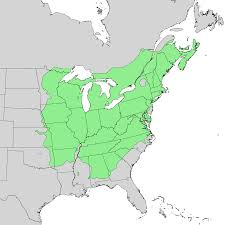
\includegraphics[width=0.5\textwidth]{qrubra_map.jpg}
\centering
\caption{Distribution map of \textit{Quercus rubra} throughout North America}
\end{figure}
\newpage
\subsection*{Description}
Quercus rubra leaves are alternate, simple with 7-11 broad lobes and are dark green and lustrous on the upper surface of the leaf. Leaves are ovate, elliptic, or obovate. The base is truncate. The lower surface is a paler green and usually hairless but can have small tufts of hair along the veins. The bark is light to medium gray and forms deep furrows with maturity. Northern red oaks have a single, straight trunk. 

There are not many known serious pest so diseases. Some oaks will form galls but they are typically harmless. Forest fires can be highly detrimental to northern red oak growth.  
\begin{figure}[ht]%
    \centering
    \subfloat[Quercus rubra Budbreak]{{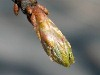
\includegraphics[width=7cm]{oak_breaking_bud.jpg} }}%
    \qquad
    \subfloat[Quercus rubra Juvenile Leaves]{{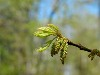
\includegraphics[width=7cm]{oak_leaves.jpg} }}%
    \caption{Quercus rubra Budbreak and First Leaves with Male Catkins}%
    \label{fig:leaves}%
\end{figure}
\newpage
\subsection*{Reproduction and Propogation}
Northern red oaks are monoecious. Male catkins burst on leaf axils that were formed from the previous year and typically break in April or May with the leaf buds. Female catkins occur with two or more spikes in the current year's leaf axils. Acorns can grow singly or in clusters of 2-5. They have shallow acorn cups and it can take 2 years to mature. Once they are mature, they will ripen and drop between August and October. This tree reaches maturity around 25 years of age, which is when flowering begins, however abundant seed production does not start until around 50 years. It is thought that the northern red oak operates in synchrony with the other oaks in the area. This synchrony is established on a temporal and spatial scale. Oaks can "communicate" with other oaks in the area in an effort to increase the overall fitness (or reproductive success) of the species. Insects or wildlife will consume or damage 80-100\% of the annual crop. Red oaks only reproduce every 2-5 years typically but occassionally they will have these masting events, where multiple oaks in the area will reproduce all at once, producing many acorns. It has been determined that oaks require a few years (i.e. 2-5 years) to recover from masting events. Similar to the predator-Prey model, which compares wolf populations to rabbit populations: as wolf populations increase, rabbit populations decrease, causing wolf populations to decrease again, and then rabbit populations to increase again, establishing this constant cycle. It is hypothesized that oaks have a similar relationship to squirrel populations: after masting events, squirrel populations boom, acorn crop yield decreases for the next couple of years, and then squirrel populations decrease again. It is this idea of synchronous ecological maintenance.
\begin{figure}[ht]%
    \centering
    \subfloat[Quercus rubra Flowers]{{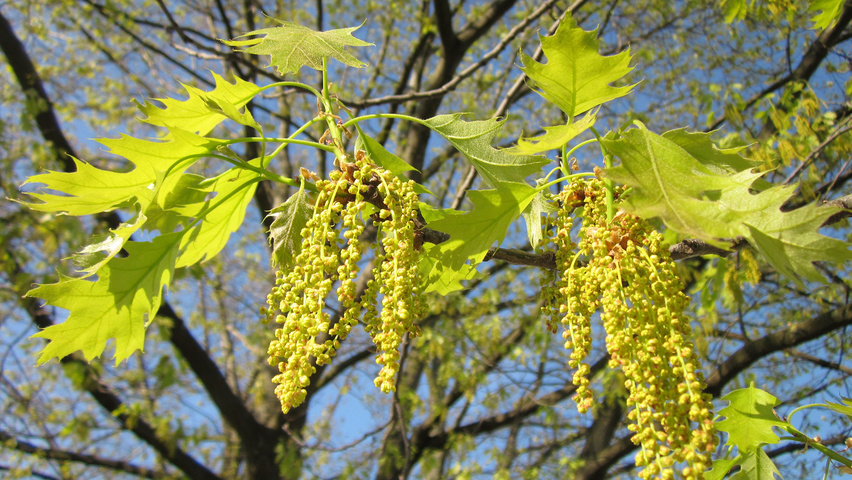
\includegraphics[width=7cm]{qrubra_flowers.jpg} }}%
    \qquad
    \subfloat[Quercus rubra Fruit]{{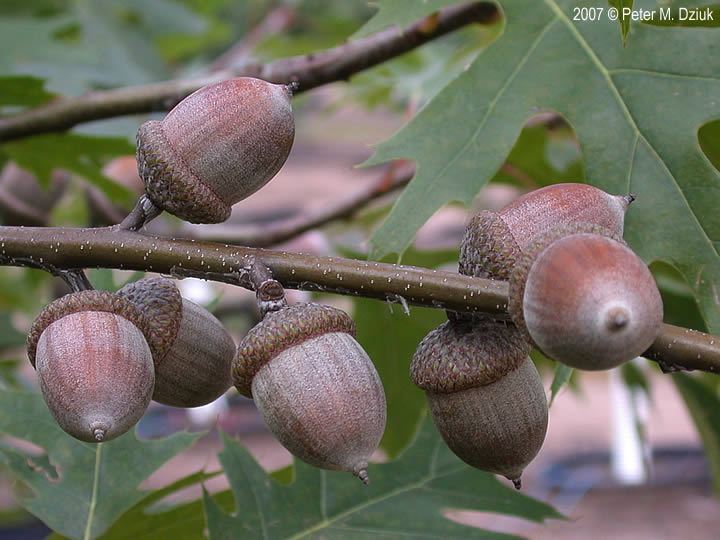
\includegraphics[width=7cm]{qrubra_fruit.jpg} }}%
    \caption{Northern Red Oak Flowers and Fruits}%
    \label{fig:fruit}%
\end{figure}
\newpage
\section*{Relation to other Oaks}
The Northern Red Oak shares a subgenus with the black oak. It is less tolerant to shade than the white or chestnut oaks but equally shade tolerant as the black and scarlet oaks. Northern red oak seedlings do not tolerate shade. 
\\
{\textbf{Interesting Facts:}}
\begin{enumerate}
\item{Northern red oaks can live as long as 300-500 years according to the USDA. However, most red oaks do not live that long today, typically 150 years.}
\item{Red oaks can reproduce from seeds or root sprouts.}
\item{They require a space in the forest canopy to reach maturity.}
\end{enumerate}
\section*{Why Study this Species?}
One of the primary reasons for the NPN choosing this species is due to its range. It is regionally distributed. By analyzing the phenological changes of the northern red oak, the NPN can pool its data and compare the differences in plant responses across the various geographical regions in the US. Like the other trees, it is also an allergen, so understanding the phenophases helps alert the public when allergen risks are higher. The NPN is also asking for volunteers to take note if there is evidence of leaf color change due to drought by making a notation in the comments section of the datasheets. 
\newpage
\section*{References}
\url{http://www.missouribotanicalgarden.org/PlantFinder/PlantFinderDetails.aspx?kempercode=i760} \\
\url{http://www.fs.fed.us/database/feis/plants/tree/querub/all.html} \\
\url{https://www.arborday.org/Trees/TreeGuide/treedetail.cfm?itemID=877} \\
\url{http://hort.ufl.edu/database/documents/pdf/tree_fact_sheets/queruba.pdf} \\
\url{http://hort.uconn.edu/detail.php?pid=378}\\
\url{https://www.na.fs.fed.us/pubs/silvics_manual/volume_2/quercus/rubra.htm}\\
\url{http://www.museum.state.il.us/muslink/forest/htmls/trees/Q-rubra.html}

\end{document}
